\originalchapter{贝塔与伽马衰变}\label{ch:beta-gamma}
\originalsection{贝塔反应与原子质量差}
$\beta^-$ 衰变 $n\to p+e^-+\bar\nu_e$ 使核 $Z$ 增一, $\beta^+$ 衰变使 $Z$ 减一并产生 $e^++\nu_e$, 电子俘获 $p+e^-\to n+\nu_e$ 同样使 $Z$ 减一. $A$ 在这些过程保持不变. 对中性原子质量,
\begin{align*}
 Q_{\beta^-}&=[M(A,Z)-M(A,Z+1)]c^2,\\
 Q_{\beta^+}&=[M(A,Z)-M(A,Z-1)-2m_e]c^2,\\
 Q_{\rm EC}&=[M(A,Z)-M(A,Z-1)]c^2.
\end{align*}
$\beta^+$ 式中的 $2m_e$ 来自正电子以及两侧中性原子的电子数差. 电子俘获还要减去被俘获电子的结合能与反冲. 不能把 $Q_{\rm EC}>0$ 自动当作 $\beta^+$ 也允许.

\originalsection{连续谱和中微子}
若只发射一个电子和反冲子核, 两体运动学会给固定电子能量. 实际 $\beta$ 谱连续, 说明至少有第三个末态粒子分享能量和动量. 近似忽略核反冲, 电子总能量 $E_e=T_e+m_ec^2$, 中微子能量 $E_\nu=Q-T_e$. 球对称动量空间态数分别正比 $p_e^2\dd p_e$ 和 $p_\nu^2\dd p_\nu$. 由 $p_e\dd p_e=E_e\dd E_e/c^2$ 及中微子近似无质量, 能量依赖为
\begin{equation}\label{eq:beta-spectrum}
 \frac{\dd\Gamma}{\dd T_e}\propto F(Z,E_e)\,p_eE_e(Q-T_e)^2\,C(E_e),\quad0\le T_e\le Q.
\end{equation}
$F$ 表示库仑畸变, $C$ 是形状因子; 允许跃迁的最低近似中 $C$ 为常数. 中微子谱通过 $T_e=Q-E_\nu$ 的变量替换取得, 不是随意把电子质量设为零.

弱相互作用的允许核跃迁可分 Fermi 与 Gamow--Teller. 前者对应同位旋算符, 核自旋变化 $\Delta J=0$; 后者还含自旋算符, $\Delta J=0,\pm1$ 但 $0\to0$ 不允许. 两者在允许近似中宇称不变. 禁戒跃迁涉及非零轻子轨道角动量与更高多极, 衰变率通常更小. ``允许''是选择规则用语, 不代表衰变一定快, 因为核矩阵元可能小.

\originalsection{电磁多极与选择规则}
核激发态发射光子时 $A,Z$ 不变. 光子的总角动量以多极阶 $L\ge1$ 分类, 角动量耦合要求 $|J_i-J_f|\le L\le J_i+J_f$. 电多极 $EL$ 的宇称因子为 $(-1)^L$, 磁多极 $ML$ 为 $(-1)^{L+1}$. 所以相同宇称的 $3/2\to1/2$ 可以发射 M1 或 E2, 奇偶改变的同一自旋变化则可以 E1 或 M2.

实光子没有 $L=0$ 模式, 因此 $0\to0$ 不能经单光子发射发生, 但可内转换或双光子过程. 低能光子长波近似满足 $kR\ll1$, 高阶多极常受 $(kR)^{2L}$ 抑制. 选择规则只给允许的矩阵元, 不能独自决定哪条核能级实际存在.

\originalsection{能级图与寿命}
利用两条相继光子线的能量之和, 可确定级联的总能差. 例如源题中 ${}^{207}\mathrm{Pb}$ 的 $897.8\,\mathrm{keV}$ 能级可经 $328.1\,\mathrm{keV}$ 与 $569.7\,\mathrm{keV}$ 级联, 中间态位于 $569.7\,\mathrm{keV}$. 把 M1、E2 性质与壳空穴模型结合, 可选出 $5/2^-$ 中间态; 单凭多极标签的全部角动量不等式有时仍允许其他组合, 壳结构是额外输入.

\begin{center}
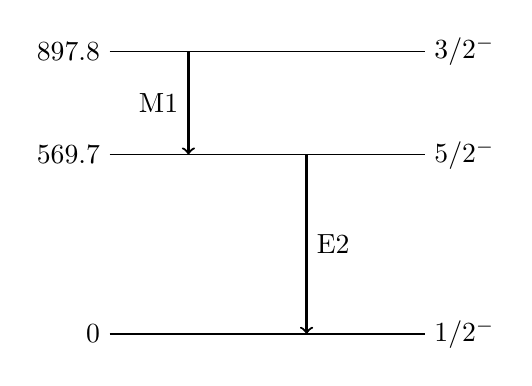
\begin{tikzpicture}[x=1cm,y=0.004cm]
\draw(0,0)--(4,0)node[right]{$1/2^-$};\draw(0,569.7)--(4,569.7)node[right]{$5/2^-$};\draw(0,897.8)--(4,897.8)node[right]{$3/2^-$};
\draw[->,thick](1,897.8)--(1,569.7)node[midway,left]{M1};\draw[->,thick](2.5,569.7)--(2.5,0)node[midway,right]{E2};
\node[left]at(0,0){$0$};\node[left]at(0,569.7){$569.7$};\node[left]at(0,897.8){$897.8$};
\end{tikzpicture}
\end{center}
图中能量单位为 keV. 长寿命核异能态可由能差小、高多极或组态矩阵元抑制造成; 它不是因核内能量守恒``暂时失效''而存在.
